\section{System Overview}
Figure~\ref{fig:framework} gives an overview of the proposed system. 
The systems assumes the mobility dataset is stored in spatial database as a Fact Table with a Star schema\cite{giovinazzo2000object,adamson2010star}. 
%To understand the Fact Table, it is important to understand the structure of the Star Schema. A traditional relational database system contains a set of tables related by primary and foreign keys. 
For instance, in our running example (i.e., NYC Taxi Trips dataset), the trips, vendors, and payment type can be represented in separate tables. A trip can have a single payment type while a payment type can be used in multiple trips. This is an example of a one-to-many relationship. 
In order to represent this data in a relational database, the $trips$ table and the $payment\_type$ table need to have a primary and foreign key. Table~\ref{tbl:fact} can be considered as the central part of the schema since it contains the foreign key to the $payment\_type$ table. Similarly, the central table also contains a foreign key in the Vendor table. Such type of schema where there is a central table consisting of facts while the remaining tables contain the meta data is called a star schema. The central table is called the Fact Table. 
%In this paper, we focuses on the Fact Table.

%The back-end of the system is spatial data manged by a spatial database. 

\begin{figure}[t]
	\centering
	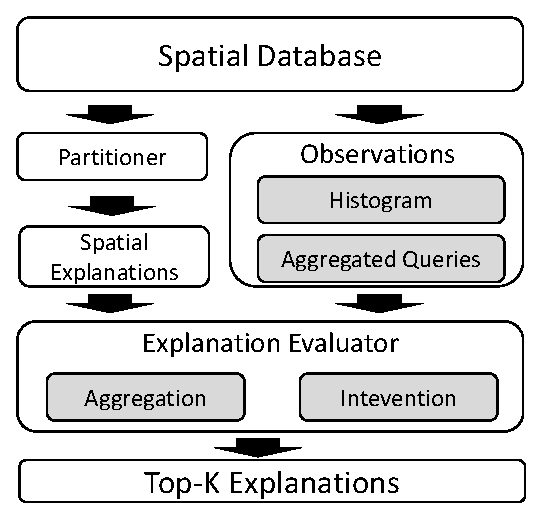
\includegraphics[width=0.4\textwidth]{images/architecture.eps}
	\caption{An outline for our system framework}
	\label{fig:framework}
\end{figure}



% \begin{center}
% \small
%   \begin{tabular}{ | l | c | }
%     \hline
%     \textbf{PaymentTypeId} & \textbf{Name} \\ \hline
%     1 & Credit Card  \\ \hline
%     2 & Cash  \\ \hline
%     3 & No Charge  \\
%     \hline
%   \end{tabular}
% \end{center}
% \captionof{table}{Payment Type Table}
% \label{tbl:payment_type}

% \begin{center}
%   \begin{tabular}{ | l | c | r | }
%     \hline
%     \textbf{StudentId} & \textbf{Name} & \textbf{Grade} \\ \hline
%     1 & John Doe & 3.2 \\ \hline
%     2 & Alice & 3.3 \\ \hline
%     3 & Bob & 3.8 \\
%     \hline
%   \end{tabular}
% \end{center}
% \captionof{table}{Students Table}
% \label{tbl:student}

%{\bf Fact Table.} 

\begin{table}
\small
\centering
\caption{\small Trips Table. PaymentType 1, 2, and 4 represent Credit Card, Cash, and No Charge, respectively.}
  \begin{tabular}{| c | c | c | c | l |}
    \hline
    {\bf VendorID} & \textbf{pickup\_lat} & \textbf{pickup\_lng} & \textbf{PayType} & \textbf{tip (\%)} \\ \hline
    0 & 34.4 & -74.2 & 1 & 15.3 \\ \hline
    1 & 34.6 & -74.1 & 1 & 10.2 \\ \hline
    0 & 34.6 & -74.3 & 1 & 9.8 \\ \hline
    2 & 34.8 & -74.6 & 2 & 11.2 \\ \hline
    1 & 34.6 & -74.3 & 1 & 10.7 \\ \hline
    0 & 34.9 & -74.1 & 3 & 0.0 \\
    \hline
  \end{tabular}
  \label{tbl:fact}
\end{table}
%\captionof{table}{\small Trips Table. PaymentType 1, 2, and 4 represent Credit Card, Cash, and No Charge, respectively.}

 %, whereas, the tables containing the meta data are called the Dimension Tables (such as the payment type table in the NYC Taxi Trip dataset).% In the case of the schema we just defined, Table.~\ref{tbl:payment_type} is the dimension table while Table.~\ref{tbl:fact} is the fact table.

Users may discover {\fact}s by querying the data stored in the spatial database. A fact can be generated from data histograms and aggregate queries. In the paper, we formally define a {\fact} $F = (Q, dir)$, where (1)~$$Q = E(q_1, q_2, .., q_m)$$ is a numeric query, where $q_i$ is a SQL query which contains an aggregate function. The aggregate function can be SUM, COUNT, or AVERAGE. So each query $q_i$ will return a single numeric value. $E$ represents a numeric expression based on the result of $q_1$, $q_2$, .., $q_m$. The operator in $E$ can be any numeric operator, such as $+$, $-$, $*$, $/$, $log$, etc. (2) $dir \in \{high, low\}$ is a direction indicating whether the user thinks the value of $Q$ is higher or lower than expected.
%For instance, the user might observe the drastic drop in the number of taxi trips on January 23, 2016 from the histogram in Figure \ref{fig:yellowstats}.
%{\bf Example.} 
For example, in Figure \ref{fig:yellowstats}, there exists a {\fact} that the number of taxi trips in NYC on January 23, 2016 dropped drastically. Such a {\fact} can be represented by two queries, $q_1$ and $q_2$ as follows:
\begin{itemize}
	\item Aggregate Query for the number of trips on January 22.
	\item Aggregate Query for the number of trips on January 23.
\end{itemize}
The difference in the number of taxi trips between the two dates can be measured by a numeric query $Q = {q_1} / {q_2}$. The number of taxi trips drops drastically, so it means the value of $Q$ is lower than the expected value. Then the {\fact} $F = ({q_1} / {q_2}, low)$.


The proposed system crunches the data to find a set of plausible explanations for an observed fact. In the paper, we formally define an {\explanation} as a predicate $\phi$, which is a conditional statement which results in a Boolean value. An {\explanation} indicates a subset of tuples in the data table which satisfy the predicate. For non-spatial {\explanation}, $\phi$ has the format of $[A$ $op$ $c]$, where $A$ is an attribute in the data table, $op$ can be $=$, $<$, $\leq$, $>$, $\leq$ and $c$ is a numeric value. For example, we can have an non-spatial {\explanation} as follows:
$$\phi: PaymentType = 1$$
%This {\explanation} indicates that all the data tuples that satisfy this predicate. 
The data scientist may use such {\explanation} to explain the {\fact} mentioned previously, which means that the drop on January 22$^{nd}$, 2016 can be explained by the trips which are paid using payment method of Type 1.

%As opposed to existing approaches, the proposed system takes into account the spatial aspect in mobility datasets to find more accurate and useful explanation.

As opposed to existing approaches, the proposed system takes into account the spatial aspect in mobility datasets to find more accurate and useful explanation.
%We take inputs in the form for aggregate queries. An arithmetic expression encapsulates the relationships between these queries. 
To achieve that, the system employs a data partitioning component that creates a hierarchy of spatial partitions, which represent the candidate spatial {\explanation}s. %Depending on the hierarchy that we have created and our inputs, we perform aggravation and intervention. The results of aggravation and intervention are used to in a ranking system based on an explanation index. The explanation index evaluator measures the quality of candidate explanations and outputs the top-k explanations. 
The {\evaluator} takes the candidate explanations and the {\fact} detected by the user as input, calculates the aggravation and intervention for each spatial explanation, and finally return the top-K plausible explanations as output.
%How much each explanation approach is weighted in the explanation index is under the control of the data analyst. 
%Finally, the top results are used for visualization. We have created a web-based GUI to display these kinds of explanations.



%\section{Observations}
% \begin{figure}[ht]
%   \begin{center}
%   \includegraphics[width=0.5\columnwidth]{observationexample}
%   \end{center}

%   \caption{An histogram showing an example observation}
%   \label{fig:observation_example}
% \end{figure}

%{\bf Numeric Query.} 


%\renewcommand{\lstlistingname}{Query}% Listing -> Algorithm
%\begin{lstlisting}[language=SQL, caption=Aggregate Query for the number of taxi trips on January 22, label=qry:aggregateexample1]
%SELECT COUNT(*) FROM
%FROM nyc_data
%WHERE date = 'January 22, 2016'
%\end{lstlisting}
%\renewcommand{\lstlistingname}{Query}% Listing -> Algorithm
%\begin{lstlisting}[language=SQL, caption=Aggregate Query for the number of taxi trips on January 23, label=qry:aggregateexample2]
%SELECT COUNT(*) FROM
%FROM nyc_data
%WHERE date = 'January 23, 2016'
%\end{lstlisting}

%When a table is analyzed, users may find an interesting {\fact} from the data table. This {\fact} is issued to the system with the defined format as the input. Then the system will try to find out the {\explanation} for the {\fact}.

%{\bf {\Fact}s.} {\Fact}s are features in the data that the user wants to explain. {\Fact}s are defined as arithmetic expressions over a set of aggregate queries. Let $F$ be the fact table in our star schema dataset. In the course of this document, we will be using relational algebra expressions defined by \cite{elmasri2011fundamentals} for aggregate expressions. Thus, the $\mathscr{F}$ symbol represents an aggregate function. An aggregate query is defined as:
%$$_A\mathscr{F}_B(D), A \in F$$
%$B$ is an aggregate function. $A$ is an attribute in our dataset. $D$ is the fact table. Examples of an aggregate function include SUM, COUNT, and AVERAGE.
%We use SQL to construct an example for an observation. Queries~\ref{qry:aggregateexample1} and \ref{qry:aggregateexample2} show examples of aggregate queries.

% Observations made on data can also be represented on histograms. Fig.~\ref{fig:observation_example} shows an example of an observation. The green bar on the histogram represents an aggregate query where the day is Friday.

%\renewcommand{\lstlistingname}{Query}% Listing -> Algorithm
%\begin{lstlisting}[language=SQL, caption=Aggregate Query for average tip percentage with credit cards, label=qry:aggregateexample1]
%SELECT AVG(tip_percentage) FROM
%FROM nyc_data
%WHERE payment_type = 1
%\end{lstlisting}
%\renewcommand{\lstlistingname}{Query}% Listing -> Algorithm
%\begin{lstlisting}[language=SQL, caption=Aggregate Query for average tip percentage with cash, label=qry:aggregateexample2]
%SELECT AVG(tip_percentage) FROM
%FROM nyc_data
%WHERE payment_type = 2
%\end{lstlisting}

%Using these aggregate queries we may form an observation based on the ratio of tip percentage with credit card against tip percentage with cash.
%$$observation = \frac{\textnormal{Query.~\ref{qry:aggregateexample1}}}{\textnormal{Query.~\ref{qry:aggregateexample2}}}$$


%\section{Explanations}
%{\bf {\Explanation}.} We 
% (but actually this explanation does not make sense).

%We go into more details for the formal definition of different kinds of explanations in Section~\ref{sec:taxonomy}. 
%If we consider Queries~\ref{qry:aggregateexample1} and \ref{qry:aggregateexample2} as an example. The explanation would be in the form of a predicate:
%$$tip\_percentage = 15.3$$
%
%Let $D$ be our solution space. We can define our predicate to be the function $P$. Let $X$ represent a set of attributes in our schema. Our explanation can now be formally defined as:
%
%\begin{equation}
%X|P(X):=
%    \begin{cases}
%      \text{true}, & \text{if}\ X \in D \\
%      \text{false}, & \text{otherwise}
%    \end{cases}
%\end{equation}

%Note that $P$ is an open ended function. In the case of spatial explanations, $P$ can take the form of a spatial function like $ST\_CONTAINS$ in PostGIS i.e. whether a polygon contains a point. In the non spatial context, $P$ can represent functions like 'greater than', 'less than', etc.

